\documentclass[12pt]{article}
\usepackage{ctex}
\usepackage[a4paper,left=25mm,right=25mm,top=25mm,bottom=25mm]{geometry}  
\usepackage{url}
\usepackage{graphicx}
\usepackage{float}
\usepackage{titletoc}
\usepackage{fancyhdr}


\begin{document}
% ----------------------------------------Linespread begin
\linespread{1.5}
% ----------------------------------------Linespread end
% ----------------------------------------Head begin
\pagestyle{fancy}
\fancyhead[C]{文章题目}
\fancyhead[L, R]{}
% ----------------------------------------Head end
% ----------------------------------------Title begin
\pagenumbering{Roman}
\title{\songti \zihao{2} \textbf{题目}}
\author{\fangsong \zihao{-3}作者1 \quad 作者2}
\date{}
\maketitle
% ----------------------------------------Title end
% ----------------------------------------Abstract begin
\ctexset{abstractname = {\zihao{-4}摘要}}
\begin{abstract}
    \zihao{-4}\fangsong 中文摘要\\
    \zihao{-4} \textbf{\heiti 关键字:}中文关键词1;中文关键词2
\end{abstract}
\ctexset{abstractname = {\zihao{-4}Abstract}}
\begin{abstract}
    \zihao{-4} 英文摘要 \\
    \zihao{-4} \textbf{\heiti Keywords:}英文关键词1;英文关键词2
\end{abstract}
% ----------------------------------------Abstract end
% ----------------------------------------Contents begin
\newpage
\tableofcontents
\contentsmargin{0pt}
\renewcommand\contentspage{\thecontentspage}
\dottedcontents{section}[20pt]{\vspace{1mm}\bfseries\songti\zihao{-4}}{25pt}{5pt}
\dottedcontents{subsection}[50pt]{\vspace{1mm}\songti\zihao{-4}}{30pt}{5pt}
\dottedcontents{subsubsection}[80pt]{\vspace{1mm}\songti\zihao{-4}}{40pt}{5pt}
% ----------------------------------------Contents end
% ----------------------------------------Article begin
\newpage
\pagenumbering{arabic}
\section{\songti\zihao{-4}第一部分}
\section{\songti\zihao{-4}第二部分}
\subsection{\songti\zihao{-4}第二部分第一小节}
\subsubsection{\songti\zihao{-4}第二部分第一小节第一分节}
\section{\songti\zihao{-4}第三部分}
\paragraph{\songti\zihao{-4}详例}

\songti\zihao{-4}在语句内添加公式用$a^2=b^2+c^2$来表示

\songti\zihao{-4}在语段间添加公式用$$a^2=b^2+c^2$$来表示

\songti\zihao{-4}分点可以用以下代码表示:
\begin{enumerate}
    \songti\zihao{-4}\item xxx
    \songti\zihao{-4}\item xxx
    \songti\zihao{-4}\item xxx
\end{enumerate}

\songti\zihao{-4}展示图片可以用如图1来表示:
\begin{figure}[H]
    \label{fig:图片}
    \centering
    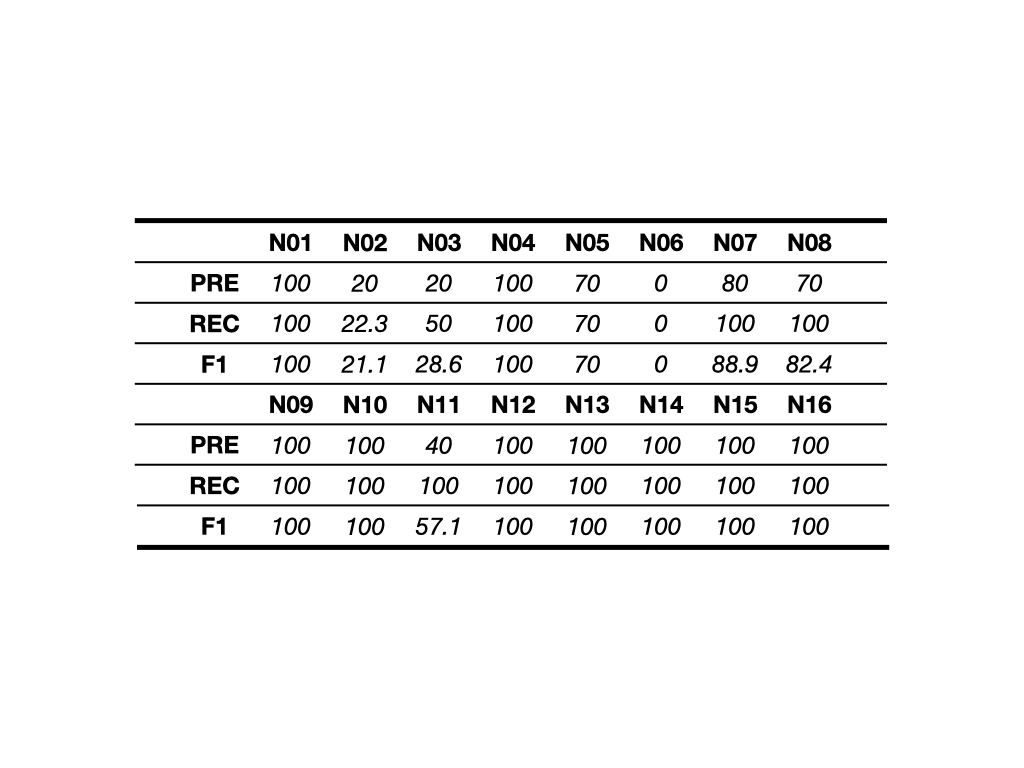
\includegraphics[scale=0.5,trim=150 220 150 220,clip]{图片.jpeg}
    \caption{\fangsong 这是一张图片}
\end{figure}

\songti\zihao{-4}展示表格可以用如表1来表示:
\begin{table}[H]
    \centering
    \begin{tabular}{ccc}
        \hline
        Parameters & T & $k_1$ \\ 
        \hline
        Values & 0.02s & 10 \\ 
        \hline
    \end{tabular}
    \caption{\fangsong 这是一个表格}
\end{table}
% ----------------------------------------Article end
\end{document}
